\chapter{Perancangan Perangkat Lunak}

Bab ini berisi tentang penjelasan perancangan perangkat lunak untuk melakukan proses \textsl{data mining} sesuai analisa yang sudah dibahas pada bab 3.

\section{Perancangan Perangkat Lunak}

\subsection{Perancangan Kelas}
Agar perangkat lunak dapat menjalankan fungsi yang sudah dibahas pada pemodelan fungsi di bab 3, maka pada subbab ini akan dibahas rancangan kelas dan \textsl{method} yang akan dibuat.

\begin{itemize}
	\item Kelas Controller, merupakan kelas untuk mengatur view dan modul ketika program dijalankan.
	\begin{itemize}
		\item Method
		\begin{itemize}
			\item public controller(), merupakan konstruktor dari kelas controller.
			\item public void startMining(String inputFilePath, String miningAlgo, JLabel label, JTextArea textArea), merupakan method untuk menjalankan modul-modul yang melakukan \textsl{data mining} dan membuat \textsl{decision tree} dari data yang menjadi masukan program.
			\item public static void main(String[] args), merupakan method main untuk menjalankan program.		
		\end{itemize}	
	\end{itemize}
	
	
	\item Kelas View, merupakan kelas untuk mengatur desain antar muka.
	\begin{itemize}
		\item Atribut
		\begin{itemize}
			\item ButtonGroup buttonGroup, digunakan untuk mengelompokkan jRadioButton.
			\item JButton buttonStart, merupakan sebuah tombol yang dapat memanggil method buttonStartActionPerformed() bila diklik.
			\item JButton buttonBrowse, merupakan sebuah tombol yang dapat memanggil method buttonBrowseActionPerformed() bila diklik.
			\item JLabel judul, merupakan sebuah label yang berisi judul dari aplikasi ini.
			\item JLabel labelFileData, merupakan label untuk menunjukkan bagian pemilihan file data \textsl{path}.
			\item JLabel labelPemilihanMethod, merupakan label untuk menunjukkan bagian pemilihan method.
			\item JLabel labelHasil, merupakan label untuk menunjukkan bagian hasil program.
			\item JLabel labelKeterangan, merupakan label untuk menunjukkan keterangan dari program.
			\item JRadioButton radioButtonId3, merupakan \textsl{radio button} yang menunjukkan bahwa user memilih method ID3 atau tidak.
			\item JRadiioButton radioButtonJ48, merupakan \textsl{radio button} yang menunjukkan bahwa user memilih method J48 atau tidak.
			\item JScrollPanel scrollPanel, merupakan variabel yang digunakan untuk mengaktifkan fungsi scroll pada JTextArea hasil.
			\item JTextArea hasil, merupakan sebuah JTextArea yang digunakan untuk menunjukkan hasil \textsl{data mining} dari program.
			\item JTextField textFieldFilePath, digunakan untuk melakukan \textsl{input path file }baik dilakukan secara manual atau melalui tombol \textsl{browse}.
			\item Controller cont, digunakan untuk memanggil \textsl{method} startMining ketika tombol buttonStart diklik.
		\end{itemize}
		\item Method
		\begin{itemize}
			\item public void buttonBrowseActionPerformed(java.awt.event.ActionEvent evt), digunakan untuk membuat jFileChooser yang berfungsi untuk memilih file dan mendapatkan \textsl{file path} dari file yang dipilih dan memasukkan \textsl{string }tersebut ke textFieldFilePath.
			\item public void buttonStartActionPerformed(java.awt.event.ActionEvent evt), digunakan untuk mengambil String dari textFieldFilePath serta method yang dipilih pada jRadioButton (Id3 atau J48) kemudian memanggil method startMining dengan masukan kedua string tersebut, label dan textArea.
		\end{itemize}
	\end{itemize}

	\item Kelas CSVReader, merupakan kelas yang memiliki method untuk membaca file dengan format CSV.
	\begin{itemize}
		\item Atribut
		\begin{itemize}
			\item ArrayList<String[]> data, digunakan untuk menyimpan isi dari file CSV yang sudah dibaca.
			\item int banyakAtribut, digunakan untuk menyimpan banyak atribut yang akan dibaca oleh CSV.
		\end{itemize}
		\item Method
		\begin{itemize}
			\item public CSVReader(), merupakan konstruktor dari kelas CSVReader.
			\item public void setEmpty, merupakan method untuk menghapus isi variabel data.
			\item public ArrayList readCSV(String file), digunakan untuk membaca file CSV.
			\item public ArrayList getData(), digunakan untuk mendapatkan variabel data.
			\item public void setData(ArrayList data), digunakan untuk mengganti nilai variabel data sesuai dengan parameter.
			\item public int getBanyakAtribut(), digunakan untuk mendapatkan nilai variabel banyakAtribut.
			\item public void setBanyakAtribut(int banyakAtribut), digunakan untuk menggati nilai variabel banyakAtribut sesuai dengan parameter.
		\end{itemize}
	\end{itemize}

	\item Kelas ProcessingData, merupakan kelas yang memiliki method untuk melakukan \textsl{preprocessing data}.
	\begin{itemize}
		\item Method
		\begin{itemize}
			\item public ProcessingData(), merupakan konstruktor dari kelas ProcessingData.
			\item public void processSorting(ArrayList array, ArrayList data, String action), digunakan untuk memilah arraylist sehingga arraylist tersebut hanya berisi \textsl{action} yang diinginkan saja (pada penelitian ini, \textsl{action} yang diharapkan adalah FINDROUTE). Hasil pilah akan disimpan pada varibel array dari parameter method sehingga tidak diperlukan return value.
			\item public ArrayList preprocessingData(ArrayList<String[]> data), Digunakan untuk melakukan tahap \textsl{preprocessing data} seperti yang sudah dijelaskan pada pemodelan data di bab 3. Tujuan dari fungsi ini adalah mendapatkan nilai waktu yang sudah diubah menjadi GMT+7 dan sudah dikelompokkan menjadi jam, hari, bulan, dan tahun serta mengetahui klasifikasi kelas dari untuk setiap \textsl{record} dengan menghitung jarak dari titik keberangkatan terhadap titik pusat Bandung dan titik tujuan terhadap titik pusat Bandung.
			\item public int KlasifikasiKelas(double jarakKeberangkatan, double jarakTujuan), Digunakan untuk menentukan kelas dari hasil jarak titik keberangkatan dengan titik pusat Bandung dan titik tujuan dengan titik pusat Bandung. 
		\end{itemize}
	\end{itemize}

	\item Kelas DecisionTree, merupakan kelas yang memiliki method untuk membuat \textsl{decision tree} dan menghitung akurasi dari pohon yang sudah dihasilkan.
	\begin{itemize}
		\item Atribut
		\begin{itemize}
			\item Classifier tree, digunakan untuk menyimpan \textsl{decision tree} yang sudah dihasilkan.
		\end{itemize}
		\item Method
		\begin{itemize}
			\item public DecisionTree(), merupakan konstruktor untuk kelas DecisionTree.
			\item public double calculatePrecision(Instances data), digunakan untuk mendapatkan nilai akurasi dari \textsl{decision tree} yang dihasilkan.
			\item public String id3(Instances data), digunakan untuk membuat \textsl{decision tree} dengan menggunakan metode ID3 dari API Weka.
			\item public String j48(Instances data), digunakan untuk membuat \textsl{decision tree} dengan menggunakan metode J48 dari API Weka.
		\end{itemize}
	\end{itemize}

	\item Kelas Dot Converter, merupakan kelas yang memiliki method untuk mengubah \textsl{string} yang merupakan hasil dari kelas DecissionTree (yaitu, \textsl{decision tree} dalam bentuk string) menjadi bahasa dot yang siap dijadikan masukan untuk graphviz.
	\begin{itemize}
		\item Method
		\begin{itemize}
			\item public String convert(String data, String miningAlgo, String nodeName), Digunakan untuk mengubah nilai string yang sudah diperoleh dari kelas DecisionTree menjadi bahasa DOT untuk membuat visualisasi dengan menggunakan graphviz.
		\end{itemize}
	\end{itemize}
\end{itemize}
	
	Pada kelas ProcessingData, nilai data waktu perlu diganti menjadi GMT+7 dan perlu menghitung jarak antar dua titik. Maka dari itu, akan dibuat dua kelas tambahan untuk melakukan kedua hal tersebut, yaitu TimezoneConverter dan DistanceHaversine.
	
\begin{itemize}
	\item Kelas TimezoneConverter, merupakan kelas yang memiliki \textsl{method} untuk mengubah waktu dari UTC menjadi GMT+7
	\begin{itemize}
		\item Method
		\begin{itemize}
			\item public static String convertToGMT7(String date), digunakan untuk mengubah waktu dari UTC menjadi GMT+7.
		\end{itemize}
	\end{itemize}

	\item Kelas DistanceHaversine, kelas yang memiliki \textsl{method} untuk menghitung jarak dua titik di bumi.
	\begin{itemize}
		\item Atribut
		\begin{itemize}
			\item double r, digunakan untuk menyimpan nilai radius dari bumi.
		\end{itemize}
		\item Method
		\begin{itemize}
			\item public double calculateDistance(double latitude1, double longitude1, double latitude2, double longitude2), Digunakan untuk menghitung jarak dari dua titik (latitude dan longitude).
		\end{itemize}
	\end{itemize}
\end{itemize}

	Setelah melakukan penelitian tentang API Weka, diperoleh bahwa input untuk membuat \textsl{decision tree} merupakan kelas Instances dari API Weka. Selain itu, diperlukan juga pengecekkan untuk hasil dari kelas tersebut, apakah sudah sesuai dengan aplikasi Weka atau belum (karena menggunakan API Weka, seharusnya \textsl{decision tree} yang dihasilkan sama). Oleh karena itu, akan ditambahkan kelas ArffIO yang berfungsi untuk menulis dan membaca data dengan format arff, sehingga ketika program melakukan \textsl{data mining}, program akan menghasilkan file dengan format .arff yang dapat dibaca oleh aplikasi Weka untuk melakukan pengetesan. Karena kita sudah memiliki file .arff tersebut, ada baiknya jika menggunakan fungsi membaca arff dari API Weka yang menghasilkan \textsl{return value} berupa kelas Instances yang dapat digunakan untuk membuat \textsl{decision tree}.

\begin{itemize}
	\item Kelas ArffIO, merupakan kelas yang berfungsi untuk melakukan penyimpanan dan membaca data dengan format arff.
	\begin{itemize}
		\item Method
		\begin{itemize}
			\item public ArffIO, merupakan konstruktor dari kelas ArffIO.
			\item public void writeArffIO(String name, ArrayList<int[]> data), digunakan untuk menulis file .arff sesuai data pada parameter.
			\item public Instances arffRead(String name), digunakan untuk membaca file .arff dengan menggunakan \textsl{method} dari API Weka.
		\end{itemize}
	\end{itemize}
\end{itemize}

Ketika mulai merancang \textsl{method} convert yang berada di kelas DotConverter, akan lebih mudah jika dirancang menjadi rekursif. Karena data yang diolah pada \textsl{method}
tersebut cukup banyak dan diperlukan nama yang berbeda pada setiap node yang akan ditulis pada DOT, maka perlu ditambah kelas yang berfungsi untuk struktur data pada kelas tersebut, yaitu SDForConvertTree.

\begin{itemize}
	\item kelas SDForConvertTree, kelas yang berfungsi untuk menyimpan data yang dibutuhkan untuk mengubah String hasil dari kelas DecisionTree menjadi bahasa DOT.
	\begin{itemize}
		\item Atribut
		\begin{itemize}
			\item String[] data, digunakan untuk menyimpan nama-nama atribut yang akan diubah ke dalam bahasa DOT.
			\item int[] count, digunakan untuk menghitung penggunaan nama setiap atribut sehingga dapat menghasilkan nama node yang berbeda untuk setiap atribut.
		\end{itemize}
		\item Method
		\begin{itemize}
			\item public SDForConvertTree(String[] data), merupakan konstruktor untuk kelas ini dan akan melakukan inisialisasi data pada atribut dengan nilai data pada parameter serta melakukan inisialisasi nilai variabel count dengan 0.
			\item public void setData(String data, index int), digunakan untuk mengubah nilai data pada index tertentu.
			\item public String[] getData(), digunakan untuk mendapatkan nilai atribut data.
			\item public String getData(int index), digunakan untuk mendapatkan nilai data pada index tertentu.
			\item public void setCount(int count, int index), digunakan untuk mengubah nilai count pada index tertentu.
			\item public int getCount(int index), digunakan untuk mendapatkan nilai count pada index tertentu.
			\item public boolean hasNext(), digunakan untuk mengecek apakah isi dari varibel data masih ada atau tidak.
			\item public void buangArrayPertama(), digunakan untuk membuang nilai array yang pertama (index ke-0).
			\item public String getDataNumber(String atribut), digunakan untuk mendapatkan angka pada nama atribut tertentu untuk membuat nama node pada kelas DotConverter agar semua nama node berbeda.
		\end{itemize}
	\end{itemize}
\end{itemize}

Setelah melakukan \textsl{convert} dari \textsl{string} hasil dari \textsl{method} pembuatan \textsl{decision tree} dari API Weka ke bahasa Dot, maka diperlukan pemanggilan fungsi dot yang terdapat pada graphviz. Cara memanggilan fungsi tersebut yaitu dengan menggunakan \textsl{command prompt}. Maka dari itu, akan diperlukan kelas yang memiliki \textsl{method} untuk memanggil \textsl{command prompt} dan menjalankan fungsi dot tersebut, yaitu kelas CMD.


\begin{itemize}
	\item kelas CMD, merupakan kelas yang digunakan untuk memanggil \textsl{command prompt}.
	\begin{itemize}
		\item Method
		\begin{itemize}
			\item public static void makeJpgUsingDotCommand(), digunakan untuk memanggil \textsl{command prompt} dan menjalankan fungsi dot dan menghasil gambar visualisasi grafik sesuai dengan file yang menjadi masukan fungsi tersebut.
		\end{itemize}
	\end{itemize}
\end{itemize}

Karena cara yang untuk memanggil fungsi dot adalah \textsl{command prompt}, maka hasil dari \textsl{method} convert harus disimpan dalam bentuk file text agar dapat dibaca oleh \textsl{command prompt}.

Dari perancangan kelas dan \textsl{method} yang sudah dilakukan, maka akan diperoleh diagram kelas seperti pada \ref{fig:classDiagram2}

\begin{figure}[H]
\includegraphics[scale=0.5, angle =90]{Gambar/classdiagram2.jpg}
\caption[Diagram \textsl{Class} Perangkat Lunak \textsl{Data Mining Log} Histori KIRI]{Diagram \textsl{Class} Perangkat Lunak \textsl{Data Mining Log} Histori KIRI} 
\label{fig:classDiagram2}
\end{figure}

\subsection{Sequence Diagram}

Pada subbab ini, akan dijelaskan alur program dengan menggunakan \textsl{sequence diagram} pada \ref{fig:sequenceDiagram}.

Pertama, program akan menampilkan desain antar muka yang dihasilkan oleh kelas View. Kemudian user akan menulis \textsl{file path} atau memilih (dengan menggunakan tombol \textsl{browse}) \textsl{input} file pada JTextField serta memilih metode pembuatan \textsl{decision tree} (tahap  pertama). Setelah memilih file dan metode, user akan menekan tombol start, dan kelas View akan memanggil \textsl{method} startMining dari kelas controller (tahap 3-4).

Kelas Controller akan mengakses file sesuai dengan masukan \textsl{file path} dengan memanggil \textsl{method} readCSV dari kelas CSVReader dan mendapat nilai kembalian berupa arraylist (tahap 5-6). Setelah mendapatkan data dari file CSV yang dipilih, data tersebut akan dipilah dan menggambil \textsl{record} dengan \textsl{action} FINDROUTE dengan cara memanggil \textsl{method} processSorting pada kelas ProcessingData dan mengembalikan ArrayList dengan data yang sudah dipilah (tahap 7-8). Kemudian data tersebut akan dilakukan \textsl{preprocessing data} dengan cara memanggil \textsl{method} preprocessingData dari kelas ProcessingData(tahap 9).

Ketika \textsl{method} preprocessingData dijalankan, perlu mengubah nilai waktu dari UTC menjadi GMT+7 dengan cara memanggil \textsl{method} convertGMT7 dari kelas TimezoneConverter dan mengembalikan nilai bertipe Date (tahap 10-11). Setelah nilai waktu diubah, diperlukan perhitungan jarak antara dua titik dengan cara memanggil \textsl{method} calculateDistance  dari kelas DistanceHaversine dan mengembalikan nilai double yang berisi jarak dari kedua titik(tahap 12-13). Kemudian diperlukan klasifikasi kelas dari jarak yang sudah dihasilkan dengan cara memanggil \textsl{method} klasifikasiKelas dari kelas ProcessingData (tahap 14-15). Kemudian semua data yang sudah diproses akan dikembalikan dalam bentuk ArrayList(tahap 16).

Setelah didapat data yang sudah dilakukan \textsl{preprocessing data}, data tersebut akan disimpan dengan format arff dengan cara memanggi \textsl{method} writeArff pada kelas ArffIO(tahap 17). Setelah disimpan, diperlukan mengambil data dari file arff yang sudah disimpan untuk mendapatkan data dengan tipe Instance dengan cara memanggil \textsl{method}readArff(tahap 18-19).

Kemudian program akan membuat \textsl{decision tree} dengan cara memanggil \textsl{method} id3 atau j48 pada kelas DecisionTree dan mengembalikan \textsl{decision tree} dalam bentuk \textsl{String}(tahap 20-21). Setelah \textsl{decision tree} dibuat, perlu dicari nilai akurasi yang diperoleh dari \textsl{decision tree} tersebut dengan cara memanggil \textsl{method} calculatePrecision dan nilai akurasi yang dihasilkan dikembalikan dalam bentuk double(tahap 22-23).

Tahap selanjutnya adalah mengubah nilai String yang diperoleh dari \textsl{method} id3 atau j48 menjadi bahasa DOT dengan cara memanggil \textsl{method} convert pada kelas DotConverter dan akan mengembalikan nilai String(tahap 24-25). Setelah diperoleh hasil dari \textsl{method} convert, maka diperlukan \textsl{command prompt} untuk menghasilkan gambar grafik untuk melakukan visualisasi \textsl{decision tree} yang sudah dihasilkan(tahap 26-27).

Setelah gambar \textsl{decision tree} dihasilkan, maka \textsl{method} startMining akan membuat JFrame yang baru untuk memperlihatkan hasil gambar \textsl{decision tree} yang sudah diperoleh serta mengembalikan nilai String \textsl{decision tree} kepada kelas View yang akan ditampilkan di JTextArea(tahap 28-29).


\begin{figure}[H]
\includegraphics[scale=0.42, angle =90]{Gambar/sequenceDiagram.jpg}
\caption[Diagram \textsl{Class} Perangkat Lunak \textsl{Data Mining Log} Histori KIRI]{Diagram \textsl{Class} Perangkat Lunak \textsl{Data Mining Log} Histori KIRI} 
\label{fig:sequenceDiagram}
\end{figure}

\subsection{Perancangan Desain Antar Muka}

Pada subbab ini, akan diperlihatkan rancangan desain antar muka yang akan digunakan untuk program ini.

Aplikasi ini memiliki dua form untuk melakukan \textsl{data mining} dan membuat \textsl{decision tree}. Pada form pertama(dapat dilihat di \ref{fig:MU1}) disediakan JTextbox dan JButton yang digunakan untuk memilih file, JRadioButton yang digunakan untuk memilih metode pembuatan \textsl{decision tree}, JTextArea yang digunakan untuk memperlihatkan hasil \textsl{decision tree} yang diperoleh dalam bentuk String, serta JTextButton yang kedua (dengan label Start) yang digunakan untuk memulai proses \textsl{data mining}. Sedangkan form kedua, berisi gambar visualisasi \textsl{decision tree} yang sudah dihasilkan(dapat dilihat di \ref{fig:MU2}).
\begin{figure}[H]
\centering
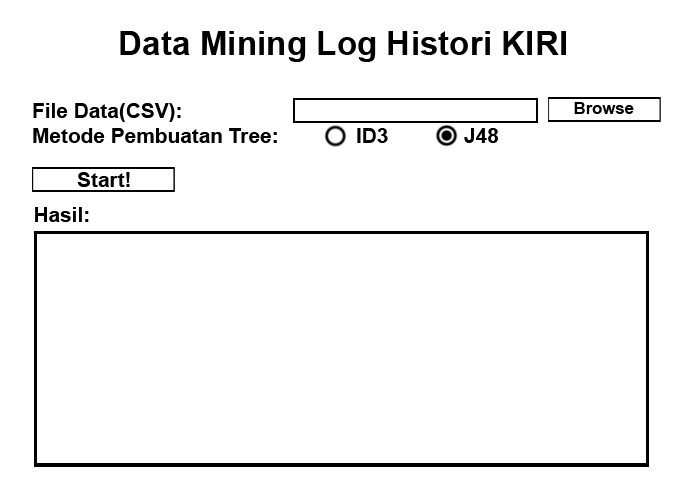
\includegraphics[scale=1.2]{Gambar/mockUp1.jpg}
\caption[Mock Up Form Pertama]{Mock Up Form Pertama} 
\label{fig:MU1}
\end{figure}

\begin{figure}[H]
\centering
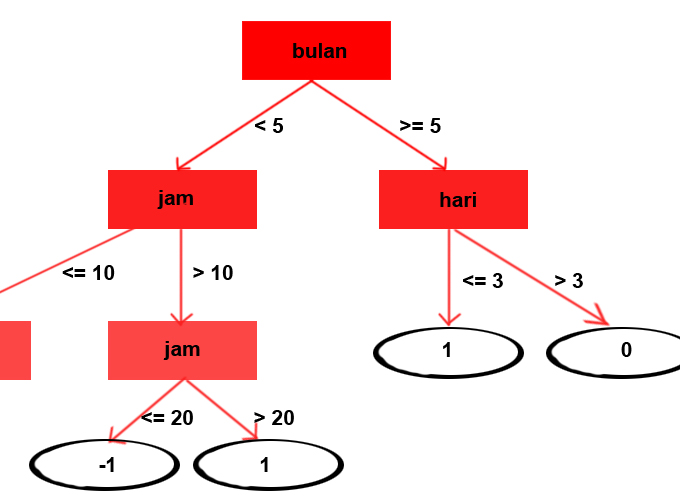
\includegraphics[scale=1.2]{Gambar/mockUp2.jpg}
\caption[Mock Up Form Kedua]{Mock Up Form Kedua} 
\label{fig:MU2}
\end{figure}